
\chapter{Lunedì 08/03/2021}
\section{Riprendiamo sullo spazio di memoria}
La differenza principale rispetto al Manchester Baby è il fatto che nelle memorie moderne è possibile accedere sia al byte che a multipli del byte. Questo comporta due questioni.
\subsection{\emph{endiannes}}
Abbiamo visto nel Manchester Baby una disposizione "strana" dei bit. Finché lavoriamo sulle singole righe, come nel Manchester Baby, non è un problema. Se iniziamo a lavorare su multipli e sottomultipli (come in tutte le architetture moderne) diventa necessario conoscere nel dettaglio come sono disposti i vari byte. Si distinguono\footnote{Satira derivante dai viaggi di Gulliver, il nome è diventato popolare in letteratura.} 
\begin{itemize}
	\item \emph{little-endian}: il byte meno significativo si trova all'indirizzo più piccolo;
	\item \emph{big-endian}: il byte più significativo si trova all'indirizzo più piccolo.
\end{itemize}
\paragraph{Rappresentazione dell'indirizzo $0x1A2B3C4D5E6F7080$}
\begin{center}
	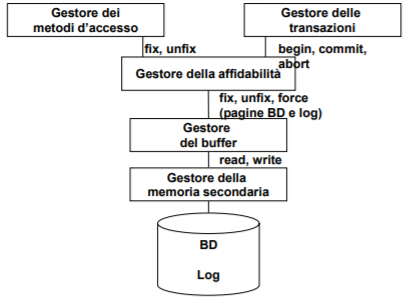
\includegraphics[scale=0.60]{img/134.PNG}
\end{center}
\paragraph{Quando nasce il problema "si fa in un modo o in un altro"?} In due occasioni:
\begin{itemize} 
	\item nascita delle reti, quindi necessità di far comunicare dispositivi con approccio diverso;
	\item nascita dell'esigenza di portare un sistema operativo da un'architettura a un'altra.
\end{itemize}
I sistemi operativi nascono normalmente per un'architettura, e sono scritti in Assembler (che è \emph{processor-specific}). UNIX è uno dei primi sistemi operativi scritti in C, rendeva possibile il passaggio da un'architettura a un'altra.  
\paragraph{Vincitori di questa guerra santa?} 
\begin{itemize}
	\item L'architettura Intel è realizzata con approccio \emph{litte-endian} (quindi noi dobbiamo ragionare così). Tutte le macchine moderne seguono questo approccio, tramite alcuni calculatori IBM professionali.
	\begin{center}
		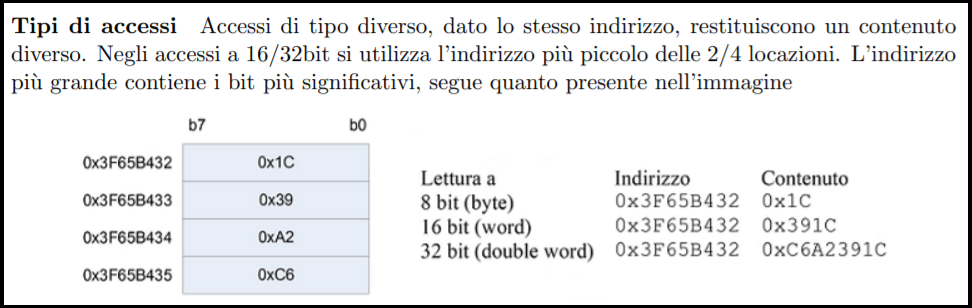
\includegraphics[scale=.65]{img/133.PNG}
	\end{center}
	\item Sulla rete ha vinto \emph{big-endian}.  Segue che un processore Intel dovrà scambiare i byte prima di inviarli.
\end{itemize}

\subsection{\emph{parallelismo}}
Quando il processore legge una parola di 8 byte il nostro interesse è leggerli tutti insieme, quindi \emph{in parallelo}. Dobbiamo organizzare la memoria in modo tale che ciò sia possibile.  
\begin{verbatim}
	MOV %AL, 1000
	MOV %AX, 1000
	MOV %EAX, 1000
	MOV %RAX, 1000
\end{verbatim}
queste operazioni scrivono tutte allo stesso indirizzo, ma pongono un numero di byte differenti. \textbf{Vogliamo evitare un tempo di esecuzione dell'istruzione proporzionale ai byte da considerare}. Un'operazione di lettura in memoria ha bisogno di più istruzioni oltre al semplice indirizzo: \underline{dobbiamo indicare anche il numero di byte coinvolti}.
\paragraph{Come vengono codificate queste informazioni dalla CPU?} Prendiamo lo spazio di memoria e \underline{dividiamolo in regioni naturali di 8 byte ciascuna} (supponiamo che la dimensione delle nostre parole sia di 8 byte). Il processore specifica 
\begin{itemize}
	\item il numero di riga (l'identificativo della regione naturale, si ignora l'offset);
	\item otto \emph{byte enabler} ($/be0, /be1, /be2, /be3, /be4, /be5, /be6, /be7$), uno per ciascuno dei byte all'interno della linea selezionata). Attraverso questi dico, data una riga formata da 8 byte, quali byte mi interessano.
\end{itemize}
\paragraph{Esempi di accessi} 
\begin{itemize}
	\item \begin{verbatim}MOV %AL, 0x3f4\end{verbatim}
		pongo $/be4=0$ e tutti gli altri uguali ad 1
		\item \begin{verbatim}MOV %AX, 0x3f4\end{verbatim}
			pongo $/be4=/be5=0$ e tutti gli altri uguali ad 1
			\item \begin{verbatim}MOV %AX, 0x3f7\end{verbatim}
				si esce dalla regione naturale. Necessario svolgere due accessi a due regioni di memoria diverse: nel primo accesso ho $/be7=0$, nel secondo $/be0=1$. Nei processori Intel la cosa è gestita automaticamente dal processore. 
			\end{itemize}
			\subsubsection{Immagine dello spazio di memoria}
			\begin{center}
				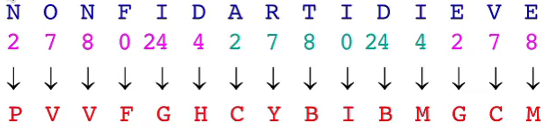
\includegraphics[scale=0.72]{img/9.PNG}
			\end{center}
			Ci conviene immaginare lo spazio di memoria come una sequenza di byte, ma organizzata in righe. Per via dell'\emph{endianess} conviene organizzare gli elementi nella direzione indicata nell'immagine. Supponiamo di avere il numero posto in fondo all'immagine: porremo le cifre meno significative nei posti con offset minore.
			
			\paragraph{Importanza dell'allineamento} Si capisce dall'ultimo esempio di accesso l'importanza dell'allineamento. Allineamento significa piazzare gli oggetti a confine di regioni grandi quanto l'oggetto. Fare questo ci garantisce che gli oggetti saranno contenuti in una stessa riga (un singolo accesso richiede centinaia di clock, quindi è importante non avere cose disallineate).
			
			\subsubsection{Organizzazione della RAM}
			\begin{center}
				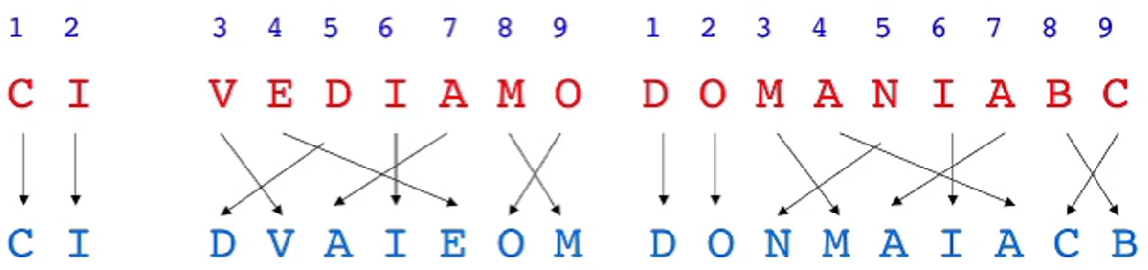
\includegraphics[scale=0.75]{img/10.PNG}
			\end{center} 
			La RAM deve essere organizzata per svolgere queste operazioni in parallelo.  
			\begin{itemize}
				\item Non possiamo collegare direttamente al bus un semplice modulo RAM con piedino di select, di lettura, e scrittura, fili di indirizzo e fili di dati. Ne dovremo collegare tanti quanti i byte che costituiscono l'intervallo. Ogni modulo rappresenta una colonna dello spazio di memoria.
				\item I moduli possono essere considerati alla pari delle RAM statiche viste a Reti logiche, ma dobbiamo tenere conto che le memorie moderne non sono fatte in quel modo. Approfondiremo la struttura circuitale delle memorie centrali moderne ad \emph{Elettronica digitale}.
				\item Abbiamo in ingresso:
				\small
				\begin{itemize}
					\item $n$ fili di indirizzo (SOLO per il numero di riga, non ho l'indirizzo completo);
					\item le variabili \emph{byte enabler}, che non vanno in ingresso a nessun circuito combinatorio (la logica combinatoria viene gestita dal processore);
					\item 64 fili di dati.
				\end{itemize}
				\normalsize
				\item I fili di dati sono ottenuti unendo insiemi di fili di dati: abbiamo $8$ fili provenienti da ciascun modulo (tanti quanti i bit che compongono il byte).
				\item Del numero di riga si fanno entrare:
				\small
				\begin{itemize}
					\item i $k$ bit meno significativi in ciascun modulo (dobbiamo dire in ciascun modulo quale elemento della colonna mi interessa, cioè quale riga);
					\item i bit rimanenti in una maschera che restituisce $0$ se la regione che vogliamo visitare si trova nel modulo RAM (non i sottomoduli, il modulo nel complesso).
				\end{itemize}
				\normalsize
				Ricordarsi, relativamente alla maschera, che lavoriamo con attivi bassi.
				\item Il valore per ciascun piedino di select è ottenuto da una porta OR che ha in ingresso l'uscita della maschera e il \emph{byte enabler} relativo\footnote{La dispensa di Lettieri pone la versione da me scritta qua (a mio parere la più intuitiva). Durante la spiegazione ha parlato di maschera con a valle una porta NOT, e di porte AND aventi in ingresso l'uscita negata della maschera e il relativo byte enabler.}.
			\end{itemize}
			\paragraph{In sostanza}
			\begin{itemize}
				\item Non si considerano i tre bit meno significativi, poichè abbiamo già i piedini \emph{byte enabler} a indicare quali posizioni ci interessano.
				\item Del numero di regione si prendono i $k$ bit meno significativi per determinare, in una colonna della RAM quale byte effettivamente ci interessa (l'offset dice cosa ci interessa orizzontalmente, i $k$ bit ciò che ci interessa verticalmente).
				\item I rimanenti bit, quelli più significativi, vanno in una maschera che determina se la RAM è interessata o no dall'operazione di lettura/scrittura (ricordare che tutte le componenti dell'architettura sono connesse sul bus, tutte ricevono e risponde solo chi è chiamato in causa).
			\end{itemize}
			\subsubsection{Osservazioni su lettura disallineata}  Prendiamo la seguente operazione
			\begin{verbatim}
				MOV 0x3ff, %RAX
			\end{verbatim}
			Il processore non fa solo due operazioni di lettura, ma deve anche riordinare gli elementi. Nella prima lettura avremo la parte meno significativa, nella seconda la più significativa. Dopo aver eseguito le due operazioni troveremo le parti invertite: la parte meno significativa nei byte più significativi del buffer, e così via. L'operazione è veloce e legata all'hardware (l'azione è eseguita dal processore e intrinseca nella MOV).
			\begin{center}
				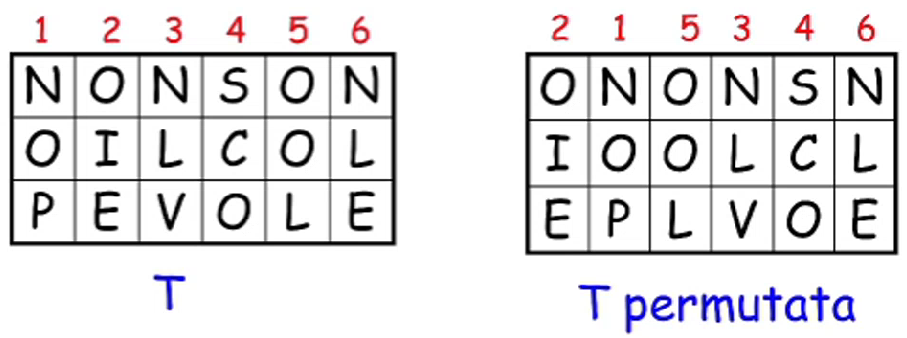
\includegraphics[scale=0.90]{img/11.PNG}
			\end{center} 
			\paragraph{Modifica di singoli bit} Per modificare un singolo bit dobbiamo
			\begin{itemize}
				\item Leggere l'intero byte
				\item Applicare una maschera con operazione logica (scegliamo la maschera in modo tale che si vada a modificare un solo bit)
				\item Scrivo il byte aggiornato
			\end{itemize}
			\begin{verbatim}
				MOV 0x3ff, %AL
				ORB $0x08, %AL <------- 00001000 OR %AL
				MOV $AL, 0x3ff
			\end{verbatim}
			In questo caso la modifica del singolo bit avviene via software. Per i dettagli ricordarsi gli esempi di operazioni viste a Reti logiche con le istruzioni macchina AND/OR/XOR.
			\paragraph{Formato di istruzioni e indirizzamento immediato} Il fatto che sorgente e destinatario non possano essere entrambi indirizzati in modo immediato è dovuto al formato di istruzioni: abbiamo spazio soltanto per un offset. L'unica alternativa è l'utilizzo di registri puntatori (nulla di nuovo rispetto a Reti logiche).